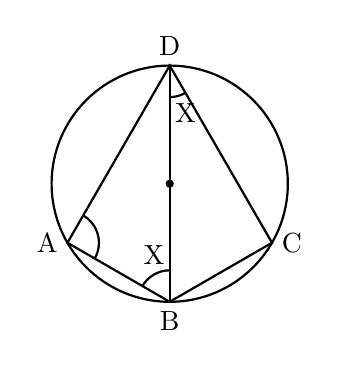
\begin{tikzpicture}[scale=1]

  % Define the center of the circle
  \coordinate (O) at (0,0);

  % Define the radius of the circle
  \def\R{1.5}

  % Draw the circle
  \draw[thick] (O) circle (\R);

  % Add a dot at the center
  \fill (O) circle (1.5pt);

  % Define the points A, B, C, D on the circle
  % D is at the top (90 degrees)
  \coordinate (D) at (90:\R);
  % B is at the bottom (270 degrees)
  \coordinate (B) at (270:\R);
  % A is on the left (approximately 210 degrees)
  \coordinate (A) at (210:\R);
  % C is on the right (approximately 330 degrees)
  \coordinate (C) at (330:\R);

  % Draw the quadrilateral ABCD
  \draw[thick] (A) -- (B) -- (C) -- (D) -- cycle;

  % Draw the vertical line segment BD
  \draw[thick] (B) -- (D);

  % Draw the angle arc at A
  % Angle from AB to AD
  % AB vector is B - A. Angle is atan2(B.y-A.y, B.x-A.x) ~ -30
  % AD vector is D - A. Angle is atan2(D.y-A.y, D.x-A.x) ~ 60
  \draw[thick] (A) +( -30:0.4) arc (-30:60:0.4);

  % Draw the angle arc at B (inside triangle ABD)
  % Angle from BA to BD
  % BA vector is A - B. Angle is 150
  % BD vector is D - B. Angle is 90
  \draw[thick] (B) +(150:0.4) arc (150:90:0.4);
  \node at (-0.2, -0.9) {X};

  % Draw the angle arc at D (inside triangle BCD)
  % Angle from DB to DC
  % DB vector is B - D. Angle is 270
  % DC vector is C - D. Angle is 300
  \draw[thick] (D) +(270:0.4) arc (270:300:0.4);
  \node at (0.2, 0.9) {X};

  % Add labels for the vertices
  \node[left] at (A) {A};
  \node[below] at (B) {B};
  \node[right] at (C) {C};
  \node[above] at (D) {D};

\end{tikzpicture}